\documentclass[12pt]{scrartcl}
\usepackage{graphicx}
\usepackage{amsmath}
\usepackage{float}
\usepackage{bm}
\PassOptionsToPackage{hyphens}{url}\usepackage{hyperref}

\usepackage{csvsimple}

\begin{document}

%Title section

\titlehead{CS department, Technion}
\subject{Introduction to Optimization and Deep Learning 236330}
\title{HW 5}
\subtitle{Training Neural Networks with SGD and Adagrad Methods}
\author{Uri Kirstein 311137095 \hfill sukirstn@campus.technion.ac.il\and Pavel Rastopchin 321082026 pavelr@campus.technion.ac.il}
\date{\today}
\maketitle

%end of title section

\section{Finding optimal learning rate}
\subsection{Log scale search}
In order to optimize the initial training rate (noted below as Alpha 0) and decay constant k, we ran the network on different values of those parameters in a log scale search. The learning rate scale runs from 0.1 to $10^-6$, while the decay constant runs from 1 (no decay) to $10^-7$.\\

We tested the different values on both the Stochastic Gradient Descent and Adagrad algorithms. In all the tests below we have used the same weights, which were generated vie the Xavier initialization method. In all tests below batch size was 32.\\
Each test was run on a train set that contains 500 points, like last exercise. We ran the optimization algorithms for 1000 epochs each. After that we used the obtained weights and biases, fed them to the network and checked the loss on the test set. The test set consists of 200 points. The training and test sets were created in an identical way.

\csvautotabular{SGD_TR_losses.csv}

\csvautotabular{Adagrad_TR_losses.csv}

Both algorithms have very similar results for every test loss. Adagrad is slightly better, but at an insignificant margin. The best (smallest) test loss is achieved for both algorithms with $\alpha_0 = 0.1$ and a decay constant of $k=10^{-5}$. In SGD the minimal test loss is 0.012546461 and in Adagrad it is 0.017895997004666164 - less than a 1\% apart. Both minima are $\sim 1.6\%$ smaller than the second smallest test loss.\\

The train loss is unsurprisingly lower for most parameter values. In many instances it is lower by several orders of magnitude, but not always. The minimum train loss is achieved at $\alpha_0=0.1$ and $k=10^{-6}$ for SGD and is 0.008323657. With Adagrad the minimal train loss is 0.010536475 and is achieved when $\alpha_0 = 0.01$ and $k=0.001$. As the test loss is the metric we truly care about, we will continue with the parameters that minimize it.\\

We note that the maximum is in an almost flat area in regards to the decay rate. We will now concentrate our effort at the parameter values where $0.01 \leq \alpha_0 \leq 0.5$ and $k = 10^{-6}$.

\subsection{Linear Search}
The tests on this part were conducted on a fresh set of parameters. We checked the following values of parameters:
\begin{itemize}
\item $\alpha_0$ = 0.01, 0.02, 0.03 ... 0.1, 0.2, 0.3 ... 0.5
\item k = $10^{-6}$
\end{itemize}

\csvautotabular{SGD_fine_TR_losses.csv}

\csvautotabular{Adagrad_fine_TR_losses.csv}\\\\

\textbf{SGD results:}
\begin{itemize}
\item \textit{Minimal test loss} - Achieved for $\alpha_0 = 0.3$. The minimal test loss is 0.002861623.
\item \textit{Minimal train loss} - Achieved for $\alpha_0 = 0.3$ as well. The minimal train loss is 0.002386384.
\end{itemize}

\textbf{Adagrad results:}
\begin{itemize}
\item \textit{Minimal test loss} - Achieved for $\alpha_0 = 0.5$. The minimal test loss is 0.003210535.
\item \textit{Minimal train loss} - Achieved for $\alpha_0 = 0.4$. The minimal train loss is 0.003427235. Note that the two maxima are close to each other in the $\alpha_0$ parameter.
\end{itemize}
Here we see that SGD gets smaller test losses than Adagrad consistently. The margin however is not big and the two algorithm exhibit similar behaviour - their losses increase and decrease together.\\
We chose to continue with the minima of SGD for two main reasons. First, in SGD the train loss and test loss minima coincide, indicating a more stable result. Second, the losses in the SGD function are lower, meaning it is likely to be the algorithm of choice so it makes more sense to maximize it.

\section{Finding optimal batch size}
Batch sizes are usually chosen to be powers of 2. Usually the minimum batch size considered is 32. We decided to do a more exhaustive search and start from 16. We also test what happens if the batch size is our entire set - 500 points.\\
All those tests were run with a different parameter initialization than tests on previous parts.

\csvautotabular{Batch_sizes.csv}\\\\

For SGD, the minimal test loss is 0.013080873522129466, for a batch size of 500 (the entire data set). The minimal training loss is 0.010383260939523572 for a batch size of 32.\\
For Adagrad, the minimal test loss is 0.0029901157137649493, for a batch size of 16. The minimal training loss is 0.0031247137395546444  for a batch size of 500.\\
Both algorithms achieve the minima for the test losses with the same choice - the entire set. They are still highly linked. Notice that while for most batch choices the difference in performance on the test set between the algorithms is small, the global minimum of Adagrad is ~75\% smaller than that of SGD. The results are similar if we look at the train set\\
\textbf{Conclusion - the chosen batch size is 500.}

\section{Shuffling the data}
Now that we have all our hyper parameters optimized we check whether shuffling the data improves our results. Up until now we used random draw to select the batch. With shuffling, we also change the order in which we see the samples between each epoch.\\
Since our optimal batch size was the entire set, not shuffling means simply seeing the same data again and again, while shuffling means seeing each time a different permutation of the data. We expect this to matter, as the learning rate is changing between epochs due to decay. This way we eliminate our bias for earlier samples and we expect the losses to decrease.\\
Again, for this part we reinitialized the parameters of our neural network.\\

\begin{verbatim}
SGD with optimal parameters, with random draw has a training loss of 
0.003075259937012187 and test loss of 0.0034291710115325587

SGD with optimal parameters, with reshuffle has a training loss of 
0.0035093220388956433 and test loss of 0.0033949180548200606

Adagrad with optimal parameters, with random draw has a training loss of 
0.001588031372696814 and test loss of 0.0016460816187726292

Adagrad with optimal parameters, with random draw has a training loss of 
0.0012244947436832116 and test loss of 0.0012998525545179875
\end{verbatim}
Reshuffling improves the test loss slightly with SGD, while unsurprisingly increasing the train loss. In Adagrad both losses decrease with shuffling. Adagrad has a test loss that is merely ~36\% of that of SGD, again proving to be the better performing algorithm for this task. Overall shuffling is beneficial.

\section{Convergence}
Now that we have all the hyper parameters set and we have decided to USE RESHUFFLE, we will have a look at the convergence of both method. Each method was run with the tuned parameters, once on the train set and once on the test set. For the test set, we use a batch size of 200 - the entire set. Again we used a different set of initialized parameters for this part of the exercise.\\

\begin{figure}[H]
	\hfill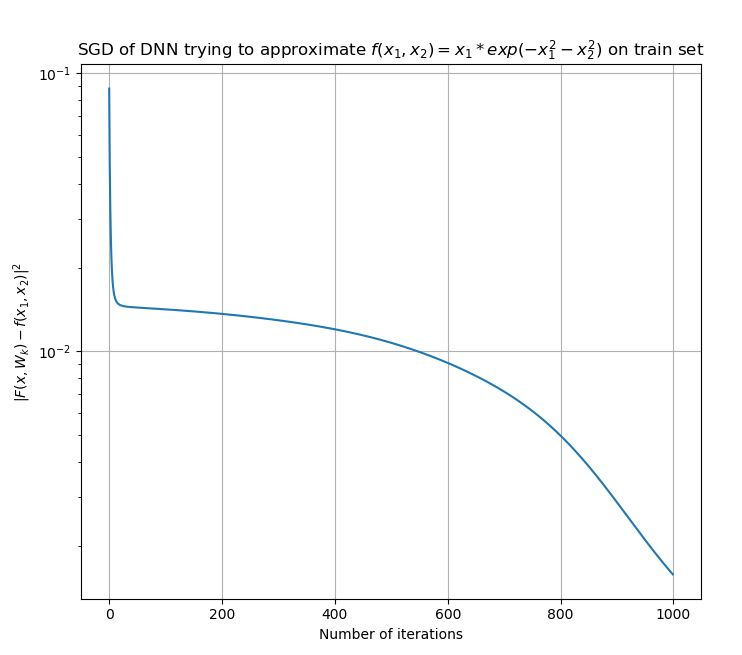
\includegraphics{SGD_train_convergence.jpg}\hspace*{\fill}
	\caption{Loss of train set as a function of epoch for the SGD algorithm}
\end{figure}

\begin{figure}[H]
	\hfill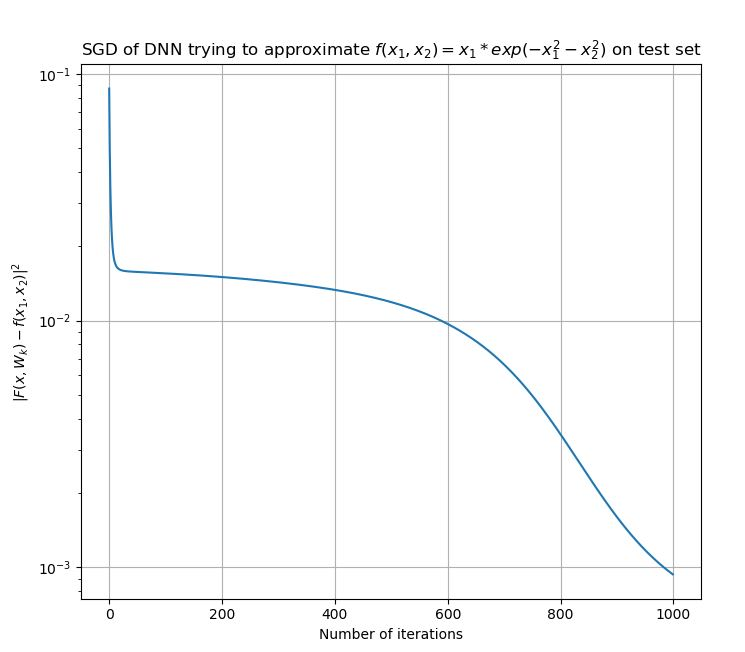
\includegraphics{SGD_test_convergence.jpg}\hspace*{\fill}
	\caption{Loss of test set as a function of epoch for the SGD algorithm}
\end{figure}

As a sanity check, indeed all algorithms and sets starts with roughly the same loss. Both SGD graphs converge very quickly in the beginning then slow down considerably, before gradually increasing the slope again. The train an test graphs for SGD have the same pot shape, but the test error is lower - this can probably be attributed to the smaller size of the test set.\\

\begin{figure}[H]
	\hfill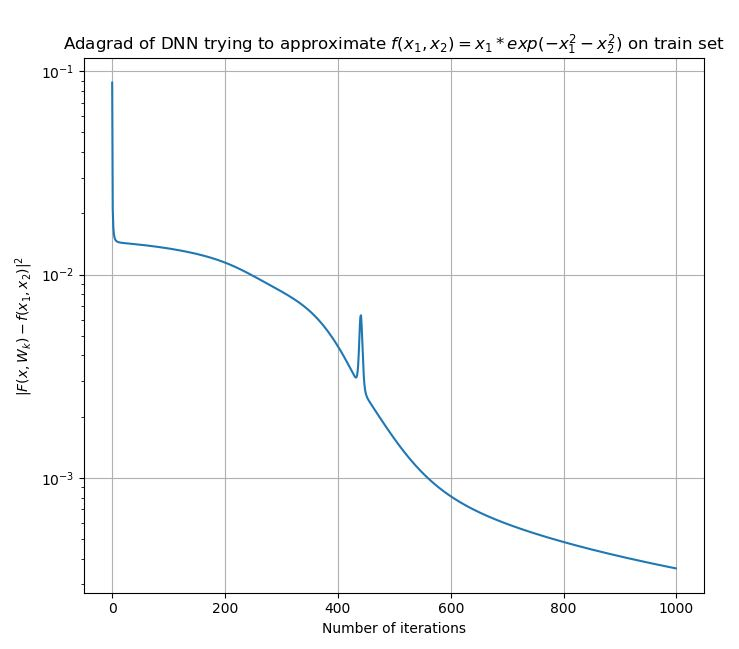
\includegraphics{Adagrad_train_convergence.jpg}\hspace*{\fill}
	\caption{Loss of train set as a function of epoch for the Adagrad algorithm}
\end{figure}

\begin{figure}[H]
	\hfill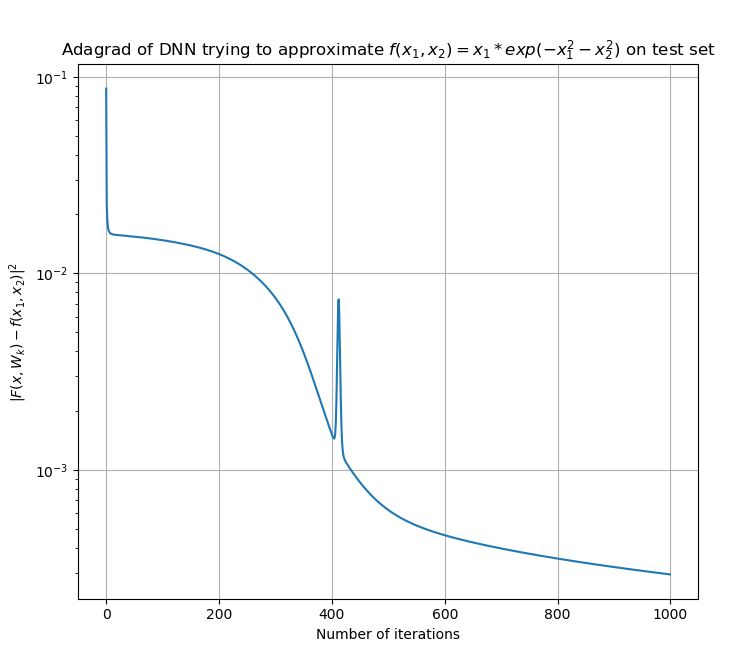
\includegraphics{Adagrad_test_convergence.jpg}\hspace*{\fill}
	\caption{Loss of test set as a function of epoch for the Adagrad algorithm}
\end{figure}

Both Adagrad graphs are similar to each other, and similar to the SGD graphs. There are two notable differences however. The first is a small local peak at around 450 for both sets. The second is the vastly better performance - by an order of magnitude. Adagrad is "stuck" for fewer epochs before picking up speed again.\\

\subsection{Comparison to FBGS}
The two algorithms are less precise than FBGS. They have higher training losses, they take more epochs to converge, if they at all do; they didn't converge after 100 epochs. However, they are vastly superior in speed.

\section{References}
\begin{itemize}
\item Log scale search - \url{https://machinelearningmastery.com/learning-rate-for-deep-learning-neural-networks/}

\item Log scale search - \url{https://towardsdatascience.com/learning-rate-schedules-and-adaptive-learning-rate-methods-for-deep-learning-2c8f433990d1}

\item Finding optimal batch size - \url{https://stats.stackexchange.com/questions/164876/tradeoff-batch-size-vs-number-of-iterations-to-train-a-neural-network}

\item Batch size search - \url{https://stats.stackexchange.com/questions/164876/tradeoff-batch-size-vs-number-of-iterations-to-train-a-neural-network}
\end{itemize}

\end{document}
